% !TEX root = main.tex

\section{Lecture 16: Form stress}
\begin{flushright}\textbf{[by Luwei Yang]}\end{flushright}

%The following relationships are commonly used in the derivation in this lecture and therefore are listed at the beginning. 

In this lecture, we derive the expression of form stress {\color{red}in the density coordinates}.

{\color{red}[Navid: this may read to someone that form-stress is an `artefact' of the particular coordinate system while, in fact, it is much more general than that... Do you agree?]}

We assume that the ocean can be divided by $N-1$ interfaces into $N$ density layers (see figure~\ref{fig:lecture16_form_stress_schematic}). 

\begin{figure}[!ht]
    \centering
    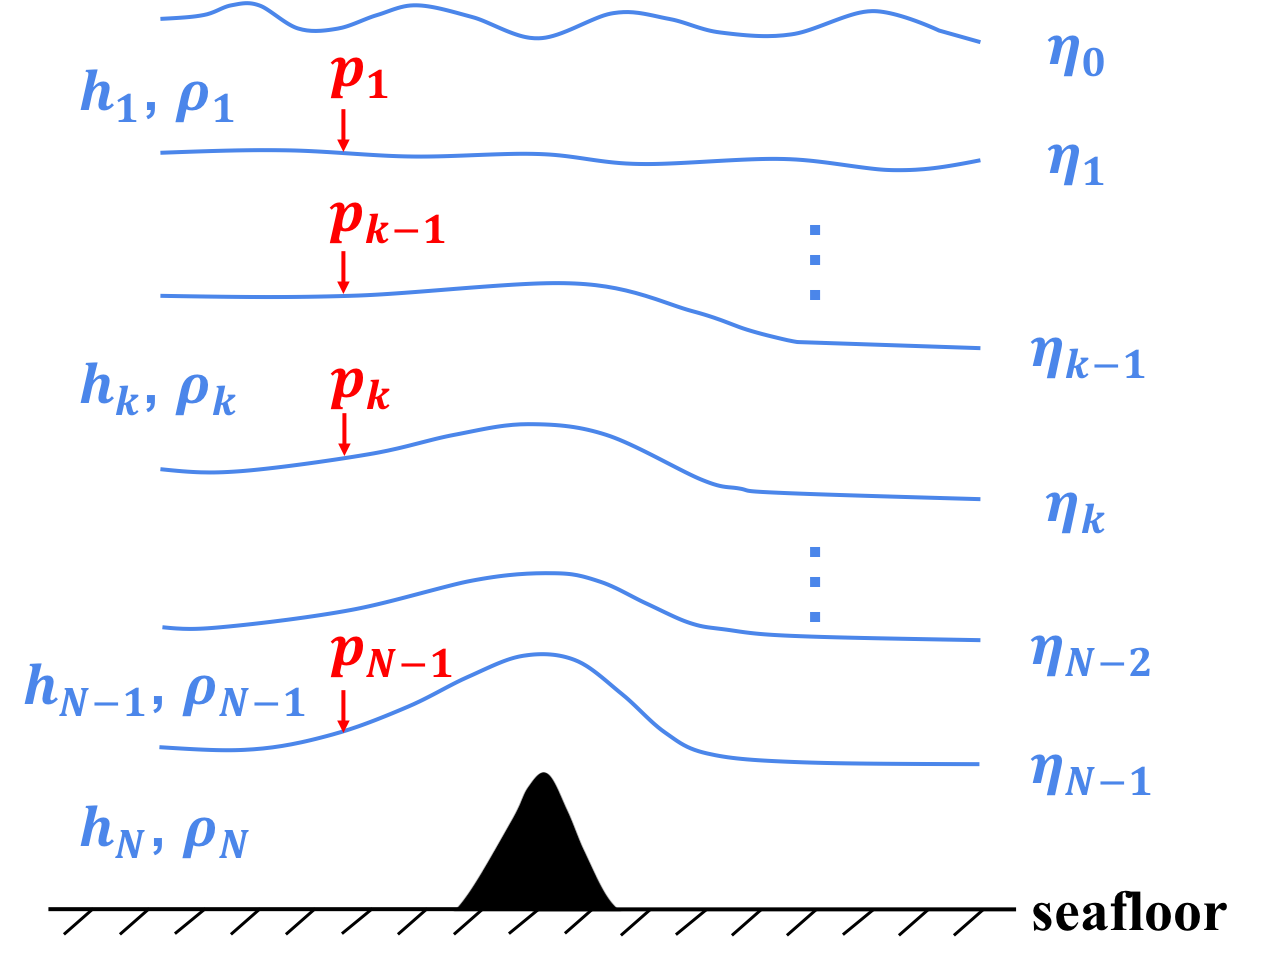
\includegraphics[width=0.6\textwidth]{lecture16_fig1}
    \caption{A schematic of density layers in the ocean.}
    \label{fig:lecture16_form_stress_schematic}
\end{figure}

We define the $k$-th layer ($k = 1, 2, \dots, N$) as the layer between the $(k-1)$-th and $k$-th interface. Under this definition, layer 1 is bounded by sea surface and the first interface, whereas the $N$-th  layer is bounded by the $(N-1)$-th interface and seafloor. The density of layer~$k$ is $\rho_{k}$. The height of the $k$-th fluid interface is denoted as $\eta_k$; $\eta_0$ is the sea surface elevation. The thickness of layer~$k$ is $h_{k}$ and satisfies
\begin{equation}
    h_{k} = \eta_{k-1} - \eta_{k}.
    \label{eq: thickness}
\end{equation}

{\color{red}[Navid: I simplified the above a bit... E.g., you had $k=1,\dots,N$ written 3-4 times...]}

The pressure felt by the $k$-th interface is $p_{k}$; the net pressure of layer $k$ is written as
\begin{equation}
    p_{k} - p_{k-1} = \rho_{k}gh_{k}.
    \label{eq: net_pressure}
\end{equation}
 
{\color{red}[Navid: OK, up to here you were just introducing definition. I think now we need 1-2 sentences of what's the plan... If you simply press on by defining $M$ and then do these algebraic acrobatics leaves one wondering where are all this is heading.... ]}
 
The Montgomery potential \textit{M} is defined as
\begin{equation}
    M = \frac{p + \rho gz}{\rho_{0}},
    \label{eq: M_def}
\end{equation}
where $p$ is pressure, $\rho$ density, $g$ the gravitational acceleration, and $\rho_{0}$ the reference density. 
The Montgomery for layer $k$ is therefore 
\begin{equation}
    M_{k} = \frac{1}{\rho_{1}}(p_{k} + \rho_{k}g\eta_{k}),
    \label{eq: M_k}
\end{equation}
{\color{red}where we use the density of first layer ($\rho_{1}$) as reference density. [Navid: do we need to use $\rho_1$ as ref density and create complications? I think this adds to the confusion. Can't we just leave it $\rho_0$? Actually the ref density should be the mean density of the fluid...]}
We also define $G_{k}$ as
\begin{equation}
    G_{k} = \frac{g\rho_{k}}{\rho_{1}}.
    \label{eq: G_k_def}
\end{equation}
The Montgomery of layer $k$ ($M_{k}$) can be rewritten as
\begin{equation}
    M_{k} = \frac{1}{\rho_{1}}\frac{1}{2}(p_{k} + p_{k-1}) + 
            \frac{1}{\rho_{1}}\frac{1}{2}(p_{k} - p_{k-1}) + G_{k}\eta_{k}.
    \label{eq: M_k_expaned}
\end{equation}
We denote the first term on the right hand side of Eq. \eqref{eq: M_k_expaned} as $P_{k}$,
\begin{equation}
    P_{k} = \frac{1}{2\rho_{1}}(p_{k} + p_{k-1}).
    \label{eq: P_k_def}
\end{equation}
The second term on the right hand side of Eq. \eqref{eq: M_k_expaned} can be rewritten by using Eq. \eqref{eq: net_pressure}, Eq. \eqref{eq: M_def}, and Eq. \eqref{eq: thickness}. Following Eq. \eqref{eq: M_k_expaned}, we then have
\begin{align}
\begin{split}
    M_{k} & = P_{k} + \frac{1}{\rho_{1}}\frac{1}{2}(p_{k} - p_{k-1}) + G_{k}\eta_{k} \\
          & = P_{k} + \frac{1}{\rho_{1}}\frac{1}{2}\rho_{k}gh_{k} + G_{k}\eta_{k} \\
          & = P_{k} + \frac{1}{2}G_{k}h_{k} + G_{k}\eta_{k} \\
          & = P_{k} + \frac{1}{2}G_{k}(\eta_{k-1} - \eta_{k}) + G_{k}\eta_{k} \\
          & = P_{k} + \frac{1}{2}G_{k}\eta_{k-1} + \frac{1}{2}G_{k}\eta_{k}
\end{split}
\label{eq: M_k_final}
\end{align}

We have derived the momentum equation ($x$-direction) for layer $k$ in Lecture~\ref{sec:lecture12}, {\color{red}[Navid: stress here that (16.9) is without any frictional terms!]}
\begin{equation}
    \frac{\partial h_{k}u_{k}}{\partial t} + \frac{\partial h_{k}u_{k}u_{k} }{\partial x} + \frac{\partial h_{k}u_{k}v_{k} }{\partial y} - f h_{k} v_{k} = - h_{k}\boldsymbol{\nabla} M_{k},
\end{equation}
or its vector form (\textcolor{red}{I don't understand how to get the vector form or what I have here is correct or not}),

{\color{red}[Navid: What do you mean? You don't understand how eqs. (16.10) and (16.9) are related?]}

\begin{equation}
    \frac{\partial h_{k}\boldsymbol{u}_{k}}{\partial t} + \boldsymbol{\nabla} ( h_{k} \boldsymbol{u}_{k} \boldsymbol{u}_{k}) + f \boldsymbol{z} \times h_{k} \boldsymbol{u}_{k} = - h_{k}\boldsymbol{\nabla} M_{k},
    \label{eq: momentum_density_coord}
\end{equation}
which shows that it is key to get an expression of $h_{k}\boldsymbol{\nabla} M_{k}$ for the derivation of form stress.
Let's expand $h_{k}\boldsymbol{\nabla} M_{k}$ using Eq. \eqref{eq: M_k_final},
\begin{align}
    \begin{split}
        h_{k}\boldsymbol{\nabla} M_{k} & = h_{k} \boldsymbol{\nabla} (P_{k} + \frac{1}{2}G_{k}\eta_{k-1} + \frac{1}{2}G_{k}\eta_{k})\\
        & = h_{k}\boldsymbol{\nabla} P_{k} + \frac{1}{2}h_{k}G_{k}\boldsymbol{\nabla} \eta_{k-1} + \frac{1}{2}h_{k}G_{k}\boldsymbol{\nabla} \eta_{k} \\
        & = \boldsymbol{\nabla} (h_{k}P_{k}) - P_{k} \boldsymbol{\nabla} h_{k} + \frac{1}{2}h_{k}G_{k} \boldsymbol{\nabla} (\eta_{k-1} + \eta_{k}) 
    \end{split}
    \label{eq: h_grad_M}
\end{align} 
Using Eq. \eqref{eq: P_k_def} and Eq. \eqref{eq: thickness}, we can rewrite the second term on the right hand side of Eq. \eqref{eq: h_grad_M} as 
$$P_{k} \boldsymbol{\nabla} h_{k} = \frac{1}{2\rho_{1}}(p_{k} + p_{k-1}) \boldsymbol{\nabla} (\eta_{k-1} - \eta_{k}). $$
Using Eq. \eqref{eq: net_pressure} and Eq. \eqref{eq: G_k_def}, we can rewrite the third term on the right hand side of Eq. \eqref{eq: h_grad_M} as
$$\frac{1}{2}h_{k}G_{k} \boldsymbol{\nabla} (\eta_{k-1} + \eta_{k}) = \frac{1}{2\rho_{1}}(p_{k} - p_{k-1}) \boldsymbol{\nabla} (\eta_{k-1} + \eta_{k}). $$
Following Eq. \eqref{eq: h_grad_M}, we have
\begin{align}
    \begin{split}
        h_{k}\boldsymbol{\nabla} M_{k} & = \boldsymbol{\nabla} (h_{k}P_{k}) - 
        \frac{1}{2\rho_{1}}(p_{k} + p_{k-1}) \boldsymbol{\nabla} (\eta_{k-1} - \eta_{k}) + 
        \frac{1}{2\rho_{1}}(p_{k} - p_{k-1}) \boldsymbol{\nabla} (\eta_{k-1} + \eta_{k}) \\ 
        & = \boldsymbol{\nabla} (h_{k}P_{k}) + 
        \frac{p_{k}}{2\rho_{1}} (\cancel{-\boldsymbol{\nabla} \eta_{k-1}} + \boldsymbol{\nabla} \eta_{k} \cancel{+ \boldsymbol{\nabla} \eta_{k-1}}  + \boldsymbol{\nabla} \eta_{k} ) + 
        \frac{p_{k-1}}{2\rho_{1}} (- \boldsymbol{\nabla} \eta_{k-1} \cancel{+\boldsymbol{\nabla} \eta_{k}} - \boldsymbol{\nabla} \eta_{k-1}  \cancel{- \boldsymbol{\nabla} \eta_{k}}) \\
        & = \boldsymbol{\nabla} (h_{k}P_{k}) + \frac{p_{k}}{\rho_{1}} \boldsymbol{\nabla} \eta_{k} - \frac{p_{k-1}}{\rho_{1}} \boldsymbol{\nabla} \eta_{k-1}.
    \end{split}
    \label{eq: h_grad_M_final}
\end{align} 
Substitute Eq. \eqref{eq: h_grad_M_final} into Eq. \eqref{eq: momentum_density_coord}, we have
\begin{equation}
    \frac{\partial h_{k}\boldsymbol{u}_{k}}{\partial t} + \boldsymbol{\nabla} ( h_{k} \boldsymbol{u}_{k} \boldsymbol{u}_{k} + h_{k} P_{k} ) + f \boldsymbol{z} \times h_{k} \boldsymbol{u}_{k} = - \frac{p_{k}}{\rho_{1}} \boldsymbol{\nabla} \eta_{k} + \frac{p_{k-1}}{\rho_{1}} \boldsymbol{\nabla} \eta_{k-1}.
    \label{eq: momentum_updated}
\end{equation}

{\color{red}[Navid: I think here the reader deserves a break. Let's add 1-2 sentences discussing eq.~\eqref{eq: momentum_updated} before heading below to an application. For example one can discuss: 1) Why was it important to do all these acrobatics so that we pulled the $h_k P_k$ term inside the divergence on the LHS? 2) What do the terms on the RHS are? Say that these terms induce momentum exchange between layers in the absence of any frictional stress! This way you can connect with the remark made regarding eq. (16.9). In my opinion that's the `amazing' thing with the form stress terms... (and also I think that's what most people have trouble digesting). ]}




For statistically steady state, the zonal average (e.g., around the Southern Ocean) of x-component of Eq. \eqref{eq: momentum_updated} yields 
\begin{equation}
    - f \overline{ h_{k}v_{k} } = \overline{ \frac{p_{k-1}}{\rho_{1}} \frac{ \partial \eta_{k-1} }{ \partial x } } - \overline{ \frac{p_{k}}{\rho_{1}} \frac{ \partial \eta_{k} }{ \partial x } },
    \label{eq: momentum_zonal_ave}
\end{equation}
Integrate Eq. \eqref{eq: momentum_zonal_ave} throughout the water column, assuming that surface buoyancy fluxes allow the water mass transformation to happen at a rate to ensure the net volume exchange across this zonal band is zero, we then obtain
\begin{equation}
    0 = \cancel{ \overline{ \frac{p_{0}}{\rho_{1}} \frac{ \partial \eta_{0} }{ \partial x } } }  - \overline {\frac{p_{N}}{\rho_{1}} \frac{ \partial \eta_{N} }{ \partial x }} + \overline{\tau_{wind}}, 
\end{equation}
where $\tau_{wind}$ is the surface wind stress, which is from the vertical integration of vertical viscous term (not shown in equations). We can rewrite the equation above as
\begin{equation}
    \overline{\tau_{wind}} = \overline{\frac{p_{N}}{\rho_{1}} \frac{ \partial \eta_{N} }{ \partial x }},
    \label{eq: momentum_zonal_ave_final}
\end{equation}
where $p_{N}$ is bottom pressure and $\eta_{N}$ the depth of the ocean. The right hand side of Eq. \eqref{eq: momentum_zonal_ave_final} is essentially the pressure difference across topography, a.k.a topographic form stress. Eq. \eqref{eq: momentum_zonal_ave_final} shows the zonally averaged momentum balance: (in the real ocean, 95\% of the) surface wind stress is balanced by topographic form stress. 
Note we ignore the contribution from bottom frictional drag to momentum balance as it is much smaller than wind stress or topographic form stress.

\textcolor{gray}{exercise will be written soon...}